\documentclass{beamer}
\beamertemplatenavigationsymbolsempty
\usetheme{Goettingen}
\setbeamertemplate{footline}[frame number]
\usecolortheme{sidebartab}

\mode<presentation>
\title[WebSocket]{Performance Evaluation of WebSocket Protocol for Implementation of Full-Duplex Web Streams}
\author{Oleg Bilovus}
\institute{Università degli Studi di Salerno}
\date[SRF 1st]{1st Scalability Research Forum}

\begin{document}
\begin{frame}
    \titlepage{}
\end{frame}

\AtBeginSection[]{ \begin{frame}\frametitle{Outline} \tableofcontents[currentsection]\end{frame} }

\section{Background}
\begin{frame}
    \frametitle{Background}
    \begin{itemize}[<+->]
        \item \emph{Historically}, creating \alert<+->{web applications} that need \alert<+->{bidirectional
                  communication} between a \alert<+->{client} and a \alert<+->{server} has required an \alert<+->{abuse of
                  HTTP to poll} the server for updates while sending upstream notifications as
              \alert<+->{distinct HTTP calls}.
    \end{itemize}
\end{frame}

\subsection{HTTP polling}
\begin{frame}
    \frametitle{HTTP polling}
    \begin{columns}
        \begin{column}{0.7\textwidth}
            \begin{figure}
                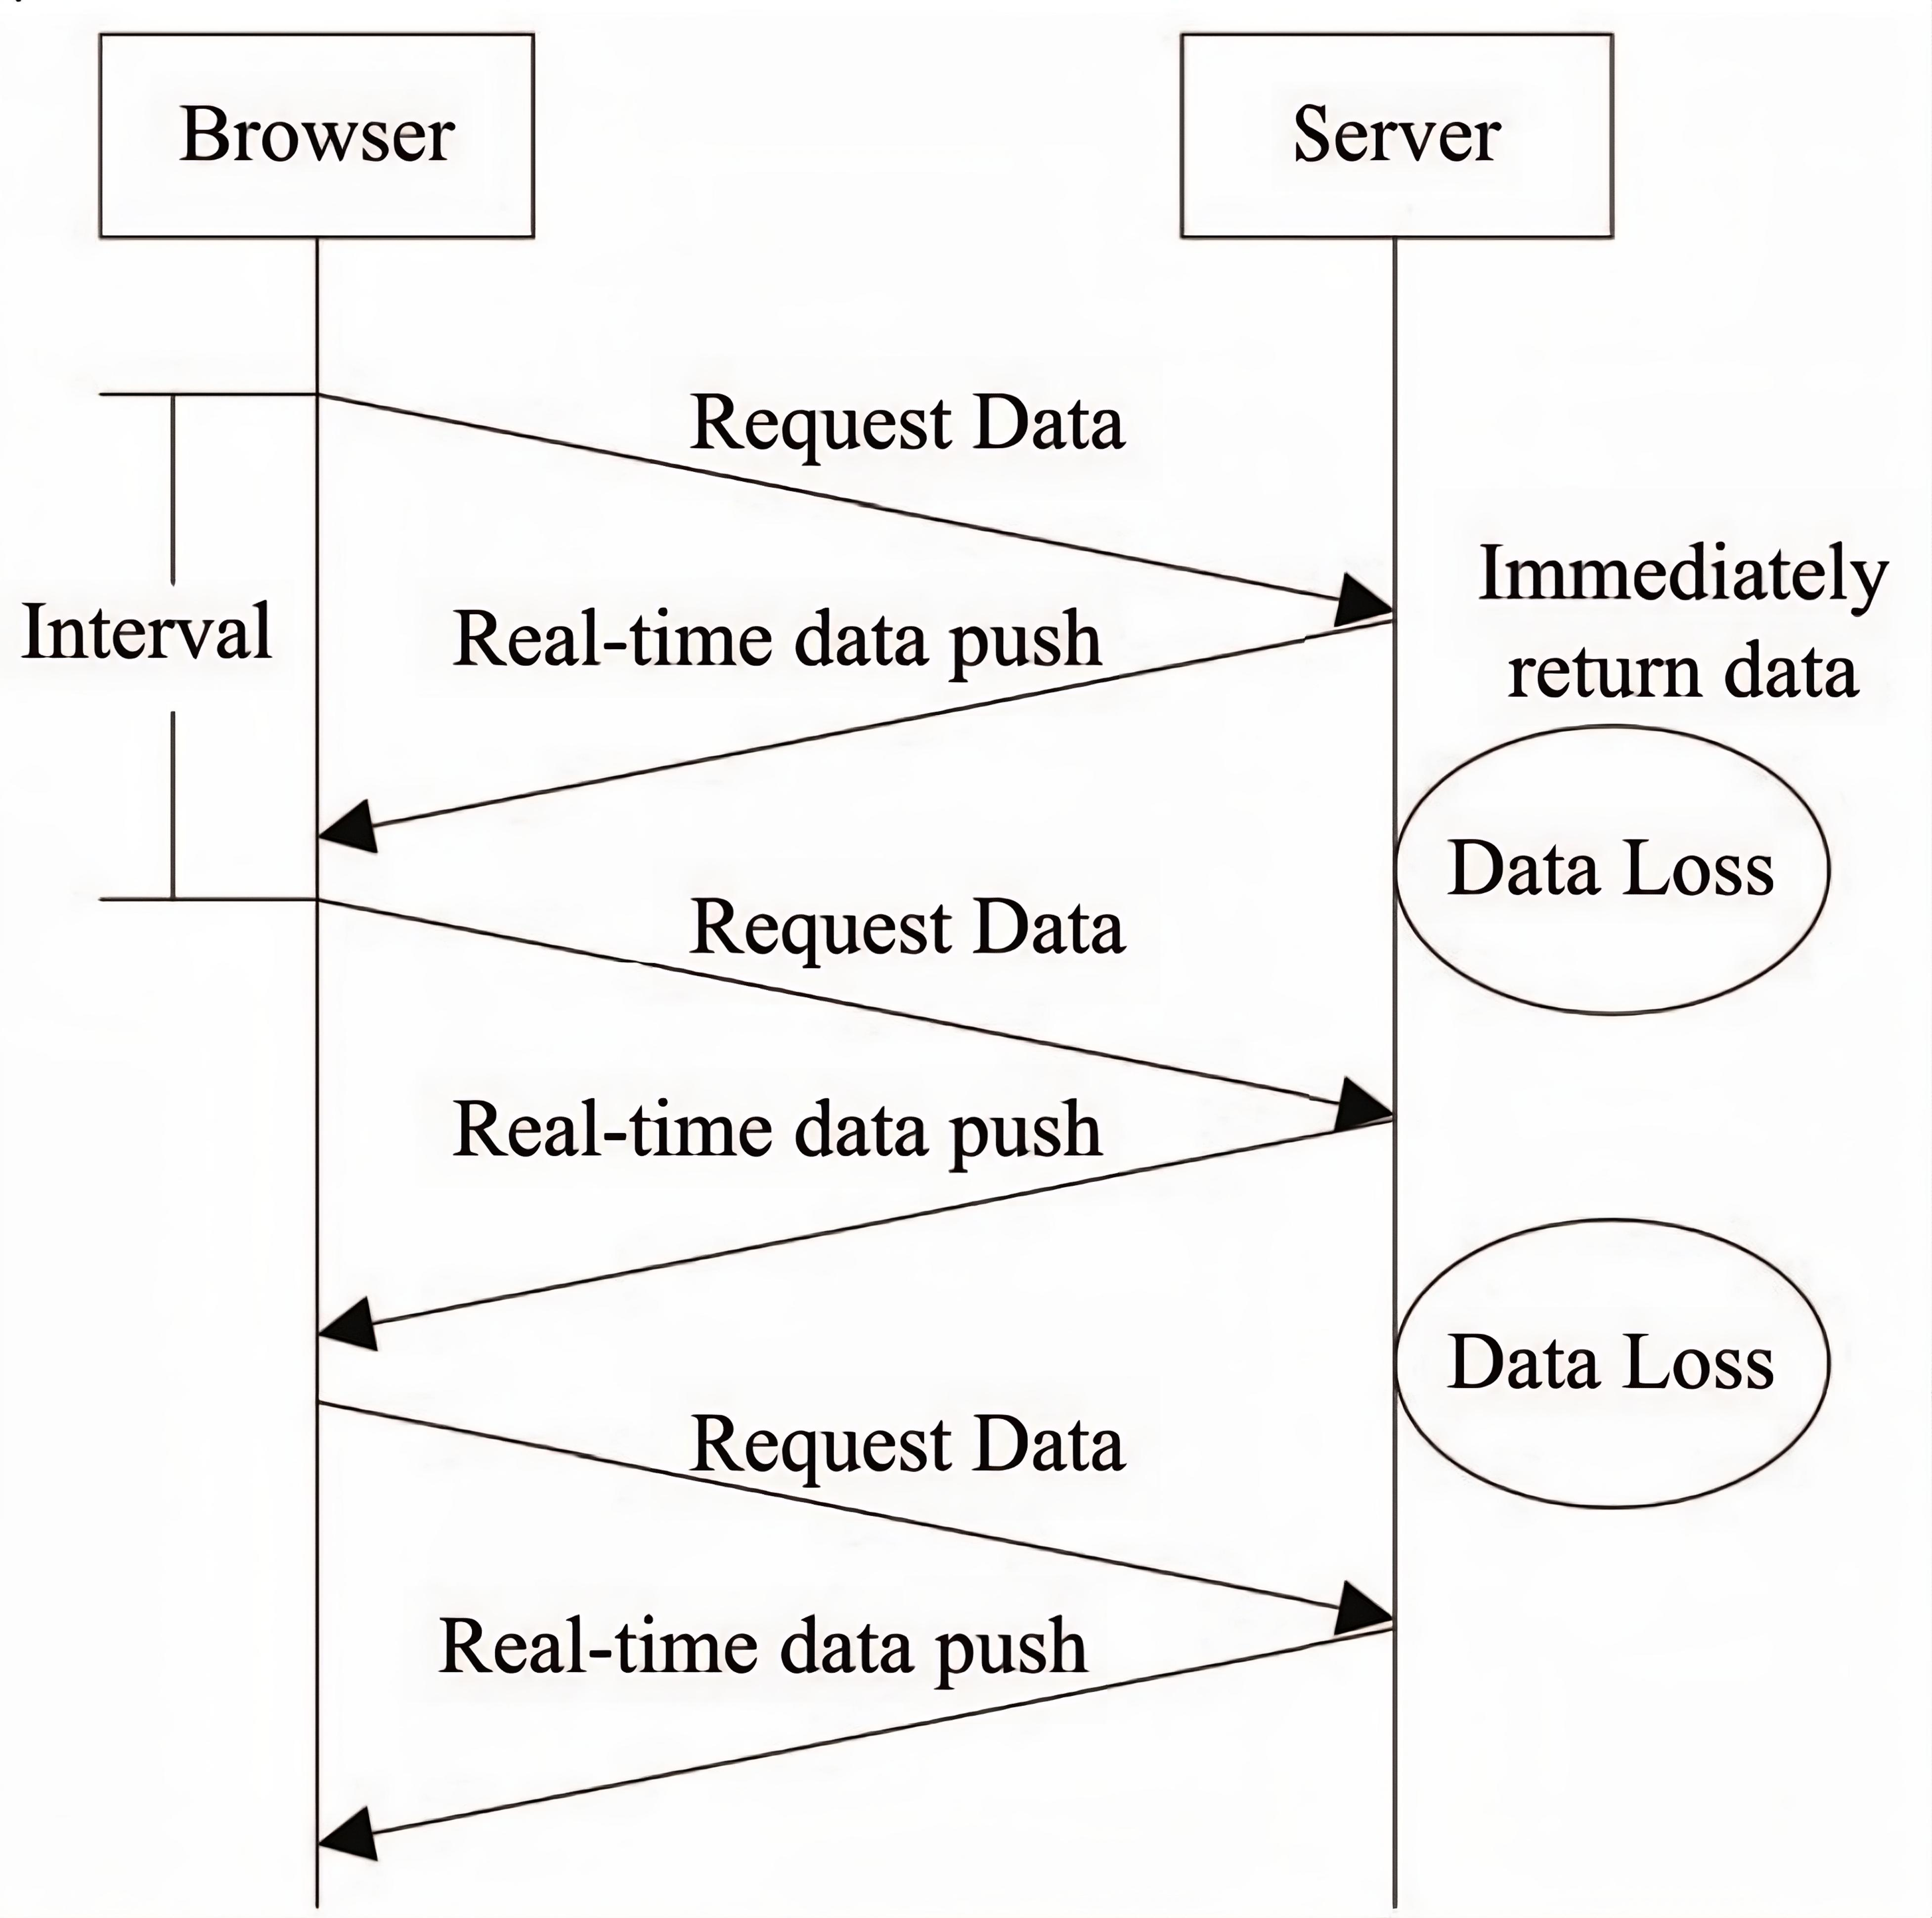
\includegraphics[width=0.7\textwidth]{images/polling.jpeg}
            \end{figure}
        \end{column}
        \begin{column}{0.4\textwidth}
            \begin{itemize}[<+->]
                \item this is a test hello hello hello
                \item this is a test hello hello hello
                \item this is a test hello hello hello
            \end{itemize}
        \end{column}
    \end{columns}
\end{frame}

\subsection{HTTP long polling}
\begin{frame}
    \frametitle{HTTP long Polling}
    \begin{columns}
        \begin{column}{0.7\textwidth}
            \begin{figure}
                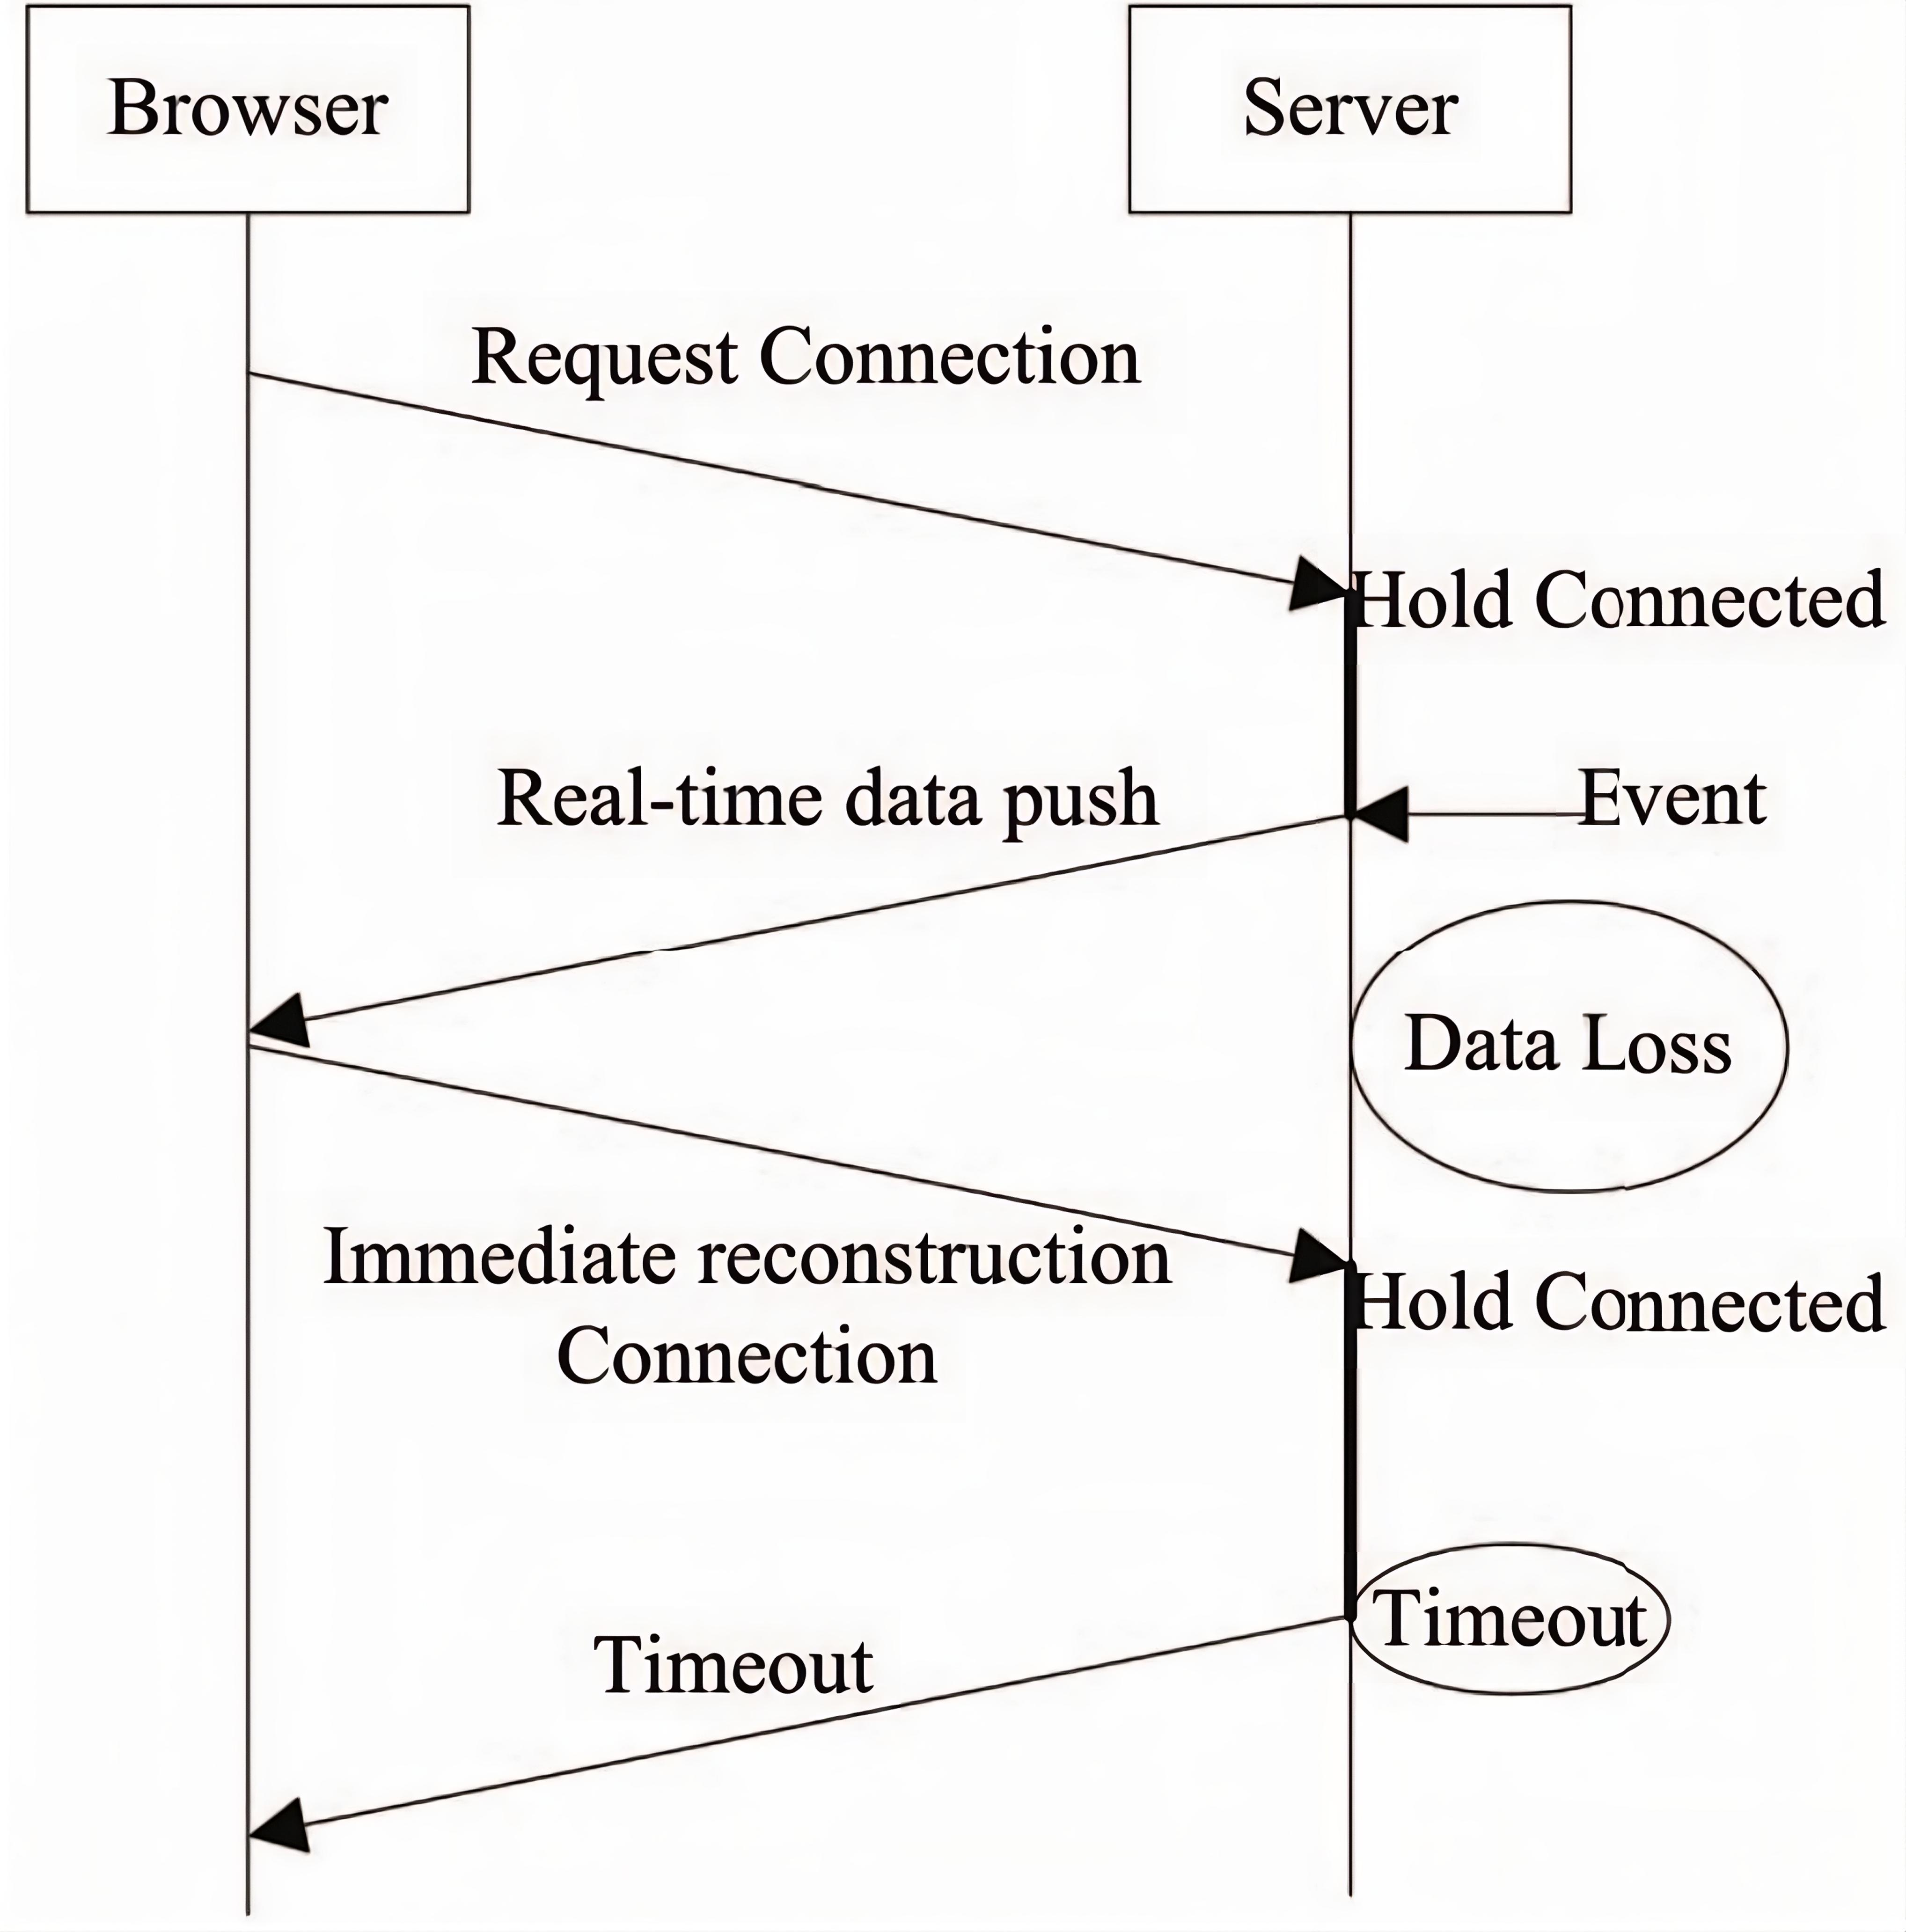
\includegraphics[width=0.7\textwidth]{images/long_polling.jpeg}
            \end{figure}
        \end{column}
        \begin{column}{0.4\textwidth}
            \begin{itemize}[<+->]
                \item this is a test hello hello hello
                \item this is a test hello hello hello
                \item this is a test hello hello hello
            \end{itemize}
        \end{column}
    \end{columns}
\end{frame}

\subsection{Streaming}
\begin{frame}
    \frametitle{Streaming}
    \begin{columns}
        \begin{column}{0.7\textwidth}
            \begin{figure}
                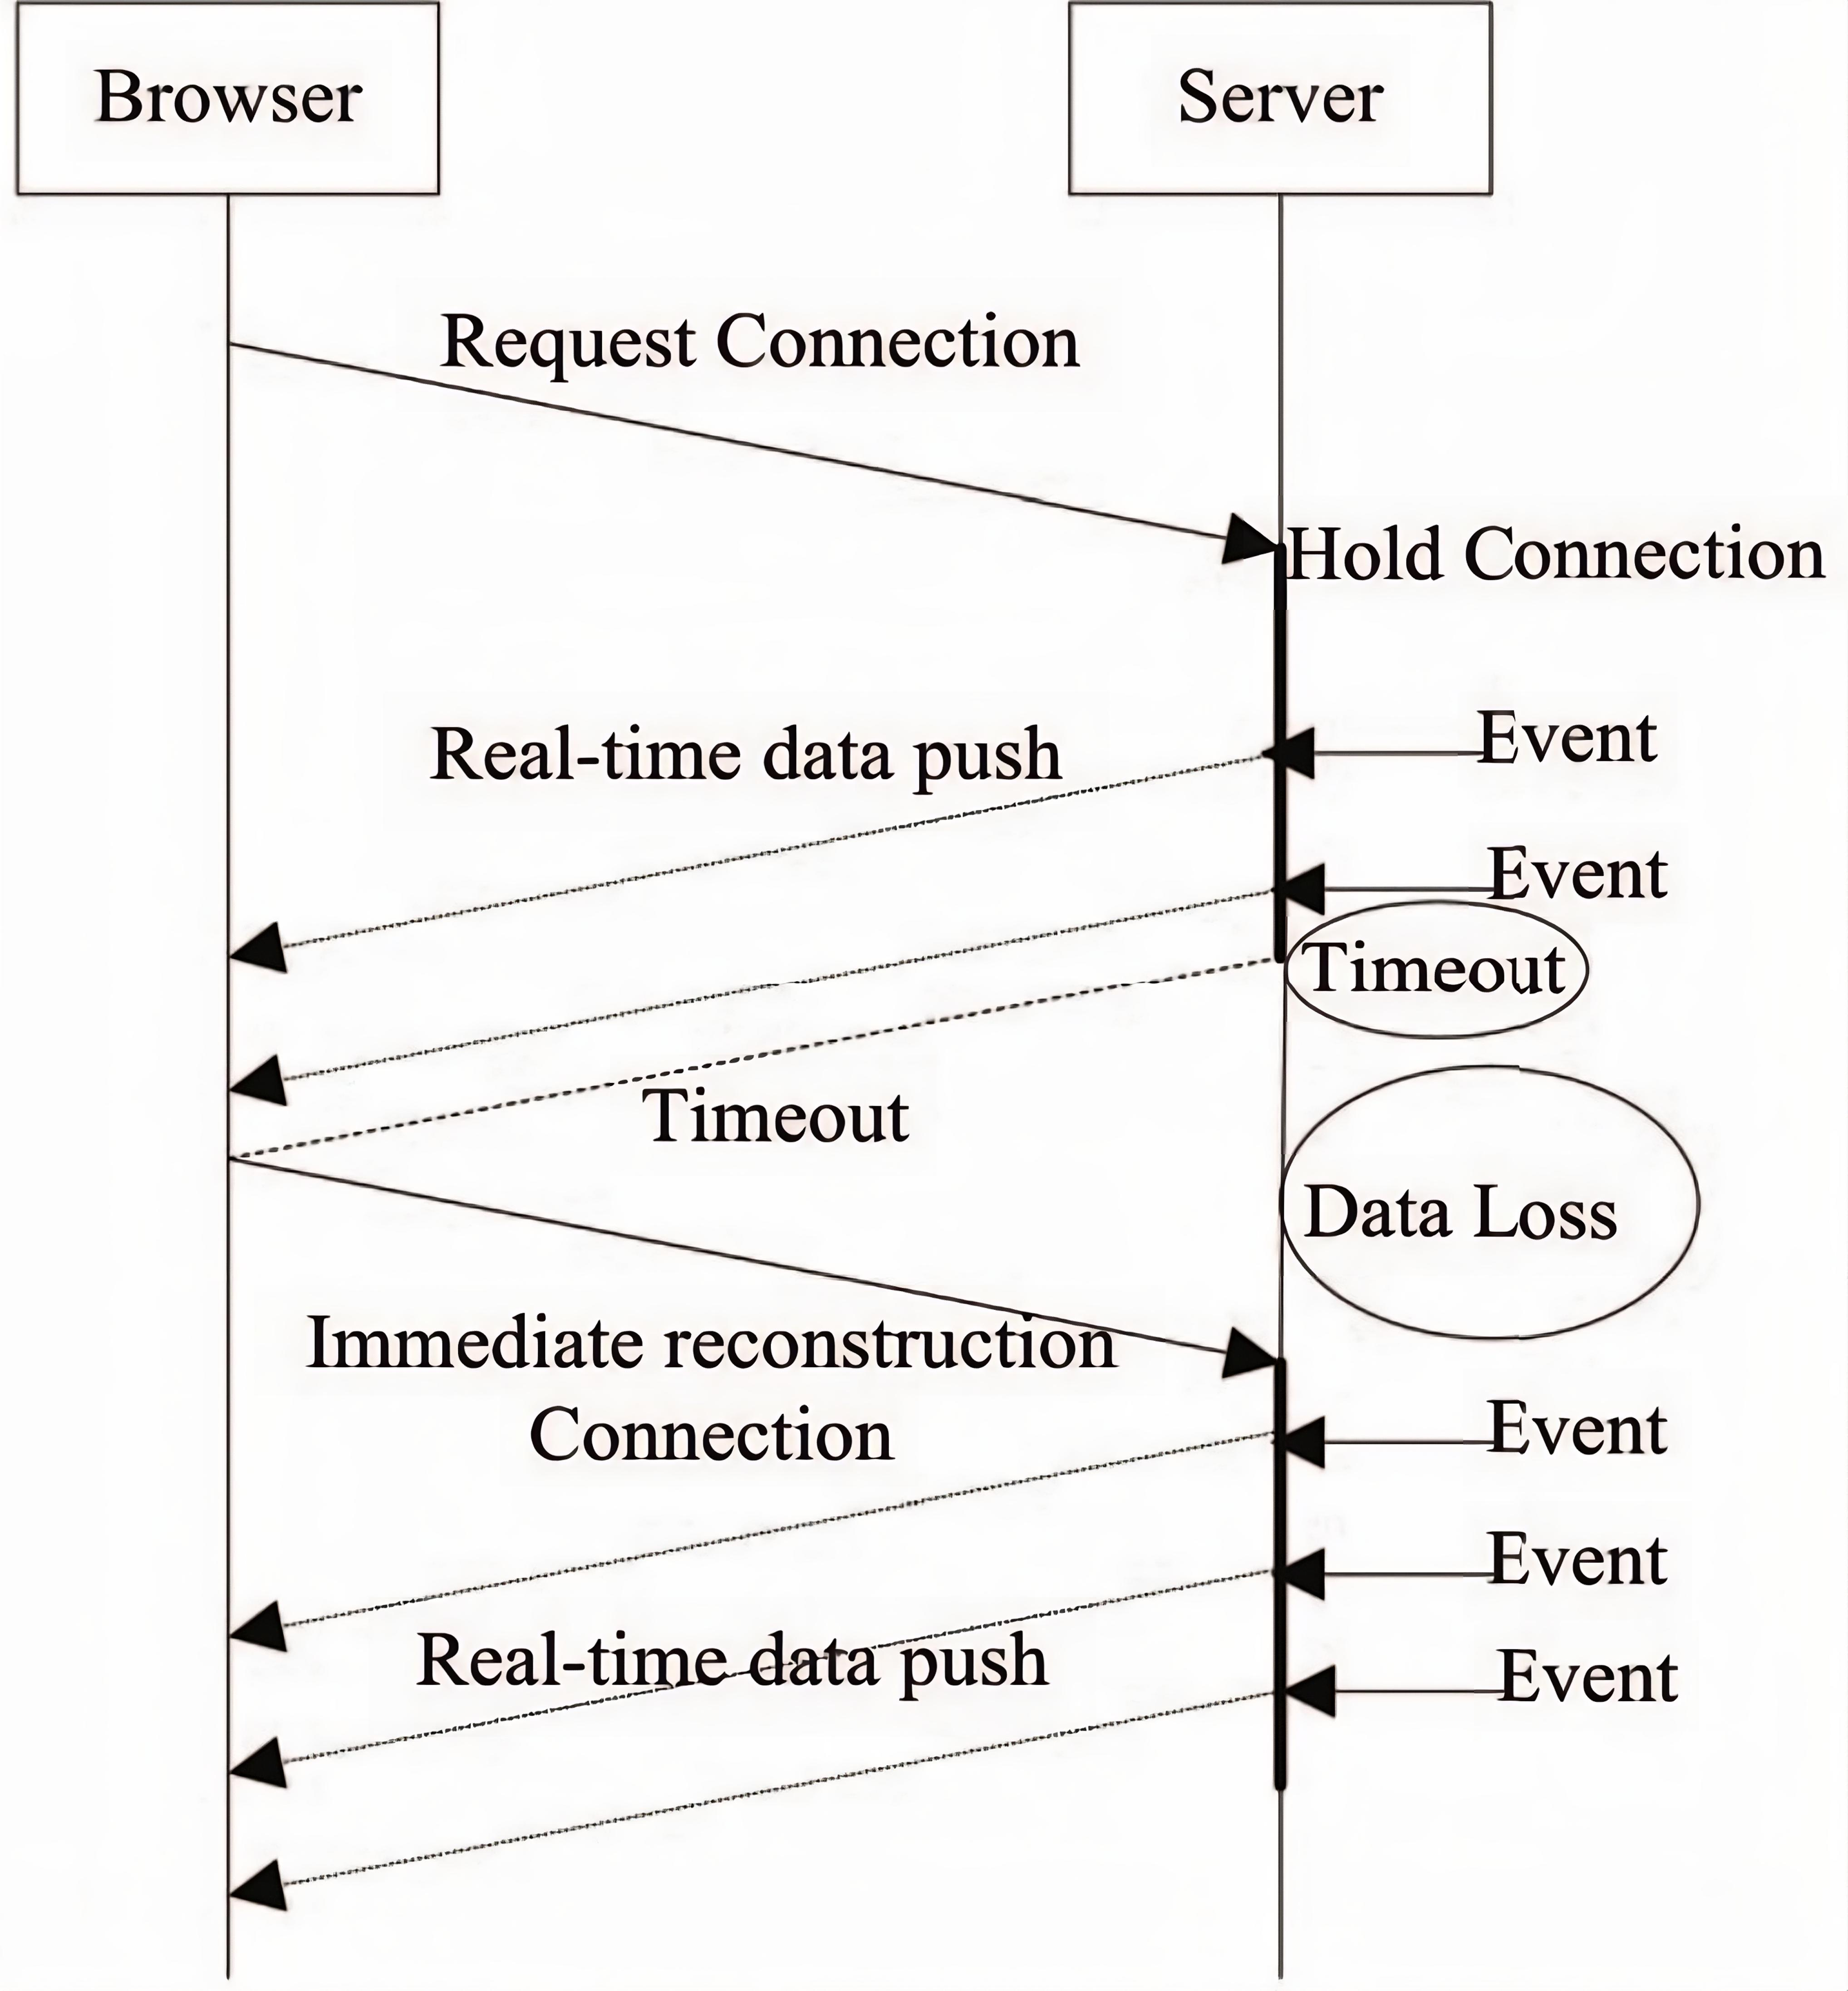
\includegraphics[width=0.7\textwidth]{images/streaming.jpeg}
            \end{figure}
        \end{column}
        \begin{column}{0.4\textwidth}
            \begin{itemize}[<+->]
                \item this is a test hello hello hello
                \item this is a test hello hello hello
                \item this is a test hello hello hello
            \end{itemize}
        \end{column}
    \end{columns}
\end{frame}

\section{WebSocket protocol}

\subsection{Definition}
\begin{frame}
    \frametitle{RFC 6455}
    \framesubtitle{Keywords}
    \begin{itemize}[<+->]
        \item The WebSocket Protocol enables \alert<+->{two-way communication} between a
              \alert<+->{client} running untrusted code in a controlled environment to a
              \alert<+->{remote host} that has \alert<+->{opted-in} to communications from
              that code.
        \item The protocol consists of an opening \alert<+->{handshake} followed by basic
              \alert<+->{message framing}, layered over \alert<+->{TCP}.
        \item The goal of this technology is to provide a mechanism for
              \alert<+->{browser-based} applications that need two-way communication with
              servers.
    \end{itemize}
\end{frame}

\end{document}